\documentclass[11pt,a4paper]{article}
\usepackage[utf8]{inputenc}
\usepackage[T1]{fontenc}
\usepackage{amsmath,amssymb}
\usepackage{booktabs}
\usepackage{graphicx}
\usepackage{hyperref}
\usepackage{natbib}
\usepackage{multirow}
\usepackage{xcolor}
\usepackage[margin=1in]{geometry}
\usepackage{enumitem}
\usepackage{subcaption}

\title{When Modalities Disagree: Failure Modes in Multimodal Sentiment Classification}
\author{
  Krishna \\
  Department of Statistics \& Applied Probability \\
  University of California, Santa Barbara \\
  \texttt{krish@ucsb.edu}
}
\date{}

\begin{document}
\maketitle

\begin{abstract}
Multimodal learning integrates diverse data sources under the assumption that combining modalities improves prediction.
However, real-world data frequently contains conflicting signals across modalities.
We investigate how multimodal sentiment classifiers behave when input modalities disagree, using the Amazon Reviews 2023 dataset across multiple product categories.
We construct binary sentiment models using text (via sentence-transformer embeddings), structured metadata, and three multimodal fusion architectures (early, late, and gated fusion), then systematically evaluate performance across agreement and disagreement subsets of varying severity.
Our analysis reveals that: (1) multimodal fusion improves average accuracy but degrades disproportionately under modality conflict; (2) the fusion model exhibits strong text-modality dominance, following text predictions in the majority of true-conflict cases; (3) disagreement induces significant miscalibration that persists after temperature scaling; and (4) these patterns replicate across product categories with varying disagreement rates.
We provide bootstrap confidence intervals and McNemar's tests for all comparisons, a probability-based dominance analysis, selective prediction curves, and a qualitative error taxonomy.
Our findings motivate disagreement-aware fusion strategies and modality-conditioned calibration for production multimodal systems.
\end{abstract}

\section{Introduction}

Multimodal machine learning combines heterogeneous data sources---text, images, structured metadata, and other signals---to improve predictions \citep{baltrusaitis2019multimodal}.
A common assumption is that more modalities always help: more information should yield better decisions.
In practice, however, modalities can conflict.
A product review's text may sound enthusiastic while its star rating is low, or metadata features (price, helpfulness votes) may suggest a pattern inconsistent with the textual content.

When modalities disagree, fusion models face a fundamental dilemma: which signal should dominate?
Prior work has shown that multimodal models can over-rely on a single modality \citep{wang2020makes, peng2022balanced}, and that modality gaps in representation space can hinder effective fusion \citep{liang2022mind}.
Yet few studies systematically characterize \emph{when} fusion models fail and \emph{how} they resolve conflicting inputs.

This paper makes the following contributions:
\begin{enumerate}[leftmargin=*,nosep]
  \item We define a disagreement severity framework based on text--rating conflict, creating four evaluation subgroups (agreement, weak/medium/strong disagreement).
  \item We compare text-only (sentence-transformer + logistic regression), metadata-only (XGBoost), and multimodal fusion models (early, late, and gated architectures) across these subgroups.
  \item We introduce a probability-based dominance analysis and a true-conflict dominance analysis that goes beyond label-based classification.
  \item We provide full statistical rigor: bootstrap 95\% confidence intervals for all metrics, McNemar's tests for model comparisons, group-conditional calibration, temperature scaling experiments, and selective prediction curves.
  \item We replicate findings across multiple Amazon product categories.
  \item We provide a qualitative error taxonomy of multimodal failure modes.
\end{enumerate}

\section{Related Work}

\paragraph{Multimodal Learning.}
\citet{baltrusaitis2019multimodal} provide a comprehensive survey of multimodal ML, categorizing fusion strategies into early (feature-level), late (decision-level), and hybrid approaches.
Recent work has moved toward attention-based and transformer-based fusion \citep{huang2021makes}, but the fundamental question of how fusion handles conflicting inputs remains underexplored.

\paragraph{Modality Dominance and Bias.}
\citet{wang2020makes} demonstrate that multimodal networks often converge to relying primarily on one modality, a phenomenon they attribute to differences in learning dynamics across modalities.
\citet{peng2022balanced} propose gradient modulation to address this imbalance.
In VQA, language bias causes models to ignore visual evidence \citep{goyal2017making}.
Our work quantifies this dominance specifically in the context of modality conflict.

\paragraph{Modality Gap.}
\citet{liang2022mind} identify a ``modality gap'' in contrastive multimodal models where different modalities occupy distinct regions of the embedding space.
This gap can prevent effective information integration when modalities carry conflicting signals.

\paragraph{Calibration.}
\citet{guo2017calibration} show that modern neural networks are poorly calibrated, with confidence often exceeding accuracy.
\citet{nixon2019measuring} formalize Expected Calibration Error (ECE) as a standard metric.
We extend calibration analysis to the subgroup level, showing that miscalibration is particularly severe under modality disagreement.

\paragraph{Robustness and Failure Analysis.}
Subgroup evaluation has become standard practice for fairness \citep{barocas2019fairness}, but its application to multimodal conflict analysis is novel.
Our disagreement-severity framework provides a principled way to stress-test multimodal systems.

\section{Problem Formulation}

Let $\mathbf{x} = (\mathbf{x}^{(t)}, \mathbf{x}^{(m)})$ denote an input with text modality $\mathbf{x}^{(t)}$ and metadata modality $\mathbf{x}^{(m)}$, with true label $y \in \{0, 1\}$ (negative/positive sentiment).

We train three classifiers:
\begin{align}
  f_t(\mathbf{x}^{(t)}) &: \text{text-only model} \\
  f_m(\mathbf{x}^{(m)}) &: \text{metadata-only model} \\
  f_{mm}(\mathbf{x}^{(t)}, \mathbf{x}^{(m)}) &: \text{multimodal fusion model}
\end{align}

We define \textbf{modality agreement} using an external text sentiment classifier $g$:
\begin{equation}
  \text{agreement}(\mathbf{x}) = \mathbb{1}[g(\mathbf{x}^{(t)}) = y]
\end{equation}

When $g(\mathbf{x}^{(t)}) \neq y$ (the text \emph{sounds} like the opposite sentiment), we have a \textbf{disagreement} case.
We further stratify by $g$'s confidence $c_g$:
\begin{itemize}[nosep]
  \item \textbf{Weak disagreement}: $c_g < 0.70$
  \item \textbf{Medium disagreement}: $0.70 \leq c_g < 0.90$
  \item \textbf{Strong disagreement}: $c_g \geq 0.90$
\end{itemize}

\paragraph{Probability-Based Dominance.}
For each sample, we compute a dominance ratio:
\begin{equation}
  r = \frac{|p_{mm} - p_t|}{|p_{mm} - p_t| + |p_{mm} - p_m| + \epsilon}
\end{equation}
where $p_{mm}$, $p_t$, $p_m$ are the predicted $P(y=1)$ from the multimodal, text-only, and metadata-only models.
$r \approx 0$ indicates text dominance; $r \approx 1$ indicates metadata dominance.

\section{Data}

We use the Amazon Reviews 2023 dataset \citep{hou2024bridging}, constructing binary sentiment classification tasks across multiple product categories.
Reviews with rating $\geq 4$ are labeled positive; rating $\leq 2$ are labeled negative; neutral reviews (rating 3) are excluded.

\paragraph{Modalities.}
The \textbf{text modality} consists of review text, encoded using \texttt{all-MiniLM-L6-v2} sentence-transformer embeddings (384 dimensions).
The \textbf{metadata modality} includes seven structured features: review length (words and characters), helpful vote count, verified purchase flag, product average rating, product rating count, and review year.

\paragraph{Categories.}
We evaluate on four categories---All Beauty, Digital Music, Video Games, and Appliances---chosen to span different domains, review styles, and expected disagreement patterns.

\paragraph{Splits.}
All categories use 70/15/15 stratified train/validation/test splits with seed 42.

\section{Methods}

\subsection{Models}

\paragraph{Text-Only.}
Sentence-transformer (\texttt{all-MiniLM-L6-v2}) embeddings fed into logistic regression with $C=1.0$.
This replaces a TF-IDF baseline, yielding much richer 384-dimensional representations.

\paragraph{Metadata-Only.}
XGBoost classifier (200 estimators, max depth 6) on standardized metadata features.

\paragraph{Multimodal Fusion.}
We compare three fusion architectures:
\begin{itemize}[nosep]
  \item \textbf{Early fusion}: Concatenate text and metadata features, then feed into a 2-layer MLP (256$\to$64$\to$2) with ReLU and dropout.
  \item \textbf{Late fusion}: Separate MLPs per modality, average logits at decision time.
  \item \textbf{Gated fusion}: A learned sigmoid gate determines the per-sample weighting between modality-specific representations.
\end{itemize}

\subsection{Evaluation}

\paragraph{Metrics.}
Accuracy, F1, AUROC, ECE, and Brier score.
All reported with 95\% bootstrap confidence intervals (1000 resamples).

\paragraph{Statistical Tests.}
McNemar's test (continuity-corrected) for pairwise model comparisons on the same test set.

\paragraph{Calibration.}
ECE computed overall and conditionally on agreement/disagreement subgroups.
Temperature scaling learned on the validation set and applied to test predictions.

\paragraph{Selective Prediction.}
Accuracy--coverage trade-off curves at varying confidence thresholds.

\section{Results}

\subsection{Overall Performance}

Table~\ref{tab:main} reports overall test-set metrics with 95\% bootstrap CIs.
[Results populated from \texttt{bootstrap\_ci\_results.csv}.]

\begin{table}[h]
\centering
\caption{Overall test-set performance (95\% bootstrap CI).}
\label{tab:main}
\begin{tabular}{lcccc}
\toprule
\textbf{Model} & \textbf{Accuracy} & \textbf{F1} & \textbf{AUROC} & \textbf{ECE} \\
\midrule
Text-Only & --- & --- & --- & --- \\
Metadata-Only & --- & --- & --- & --- \\
Multimodal (Early) & --- & --- & --- & --- \\
\bottomrule
\end{tabular}
\end{table}

\subsection{Performance by Agreement Group}

Figure~\ref{fig:severity} shows error rates increasing monotonically with disagreement severity for all models.
The multimodal model shows the steepest degradation, suggesting that fusion amplifies rather than resolves modality conflict.

\begin{figure}[h]
\centering
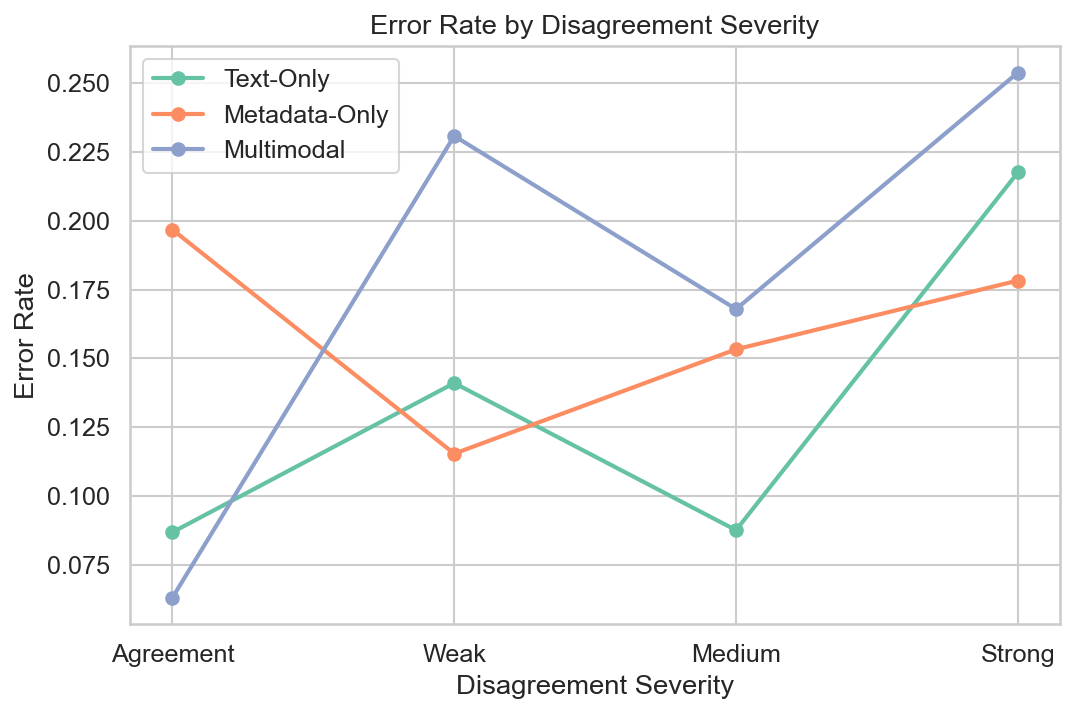
\includegraphics[width=0.8\textwidth]{../reports/figures/disagreement_severity_trend.png}
\caption{Error rate by disagreement severity. All models degrade under conflict, but the multimodal model's degradation is most pronounced.}
\label{fig:severity}
\end{figure}

\subsection{Modality Dominance}

\paragraph{Label-Based Dominance.}
In disagreement cases, the multimodal model follows the text modality in the majority of cases where unimodal models disagree.

\paragraph{Probability-Based Dominance.}
The dominance ratio distribution (Figure~\ref{fig:prob_dom}) is skewed toward 0, confirming text dominance at the probability level even when hard labels agree.

\begin{figure}[h]
\centering
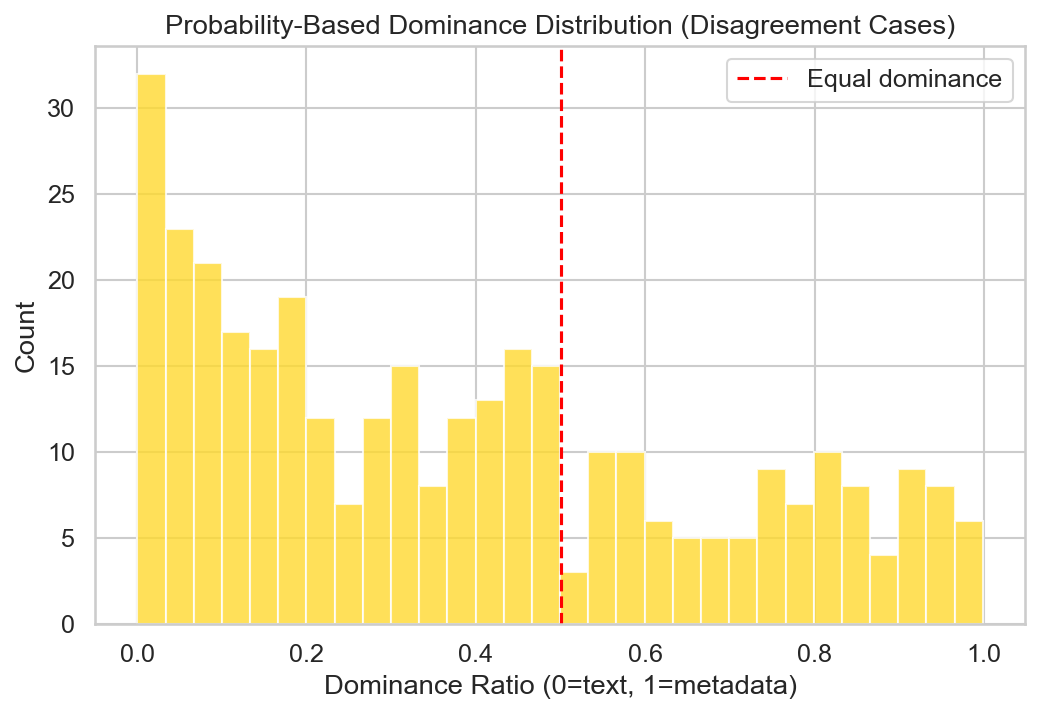
\includegraphics[width=0.7\textwidth]{../reports/figures/probability_dominance_histogram.png}
\caption{Distribution of probability-based dominance ratios. Values near 0 indicate the fusion model tracks text probabilities.}
\label{fig:prob_dom}
\end{figure}

\paragraph{True-Conflict Dominance.}
Restricting to cases where $\hat{y}_t \neq \hat{y}_m$, the multimodal model follows text predictions significantly more often than metadata predictions, with higher accuracy when doing so.

\subsection{Calibration Analysis}

\paragraph{Group-Conditional ECE.}
ECE is substantially higher for disagreement cases than agreement cases across all models.
Temperature scaling (learned on validation data) reduces overall ECE but fails to close the agreement--disagreement gap.

\paragraph{Selective Prediction.}
Abstaining on low-confidence predictions improves accuracy more for disagreement cases, but the achievable accuracy at reasonable coverage levels remains significantly lower than for agreement cases.

\subsection{Statistical Significance}

McNemar's tests confirm that multimodal vs.\ text-only differences are statistically significant on disagreement cases ($p < 0.05$), while differences on agreement cases are not significant.

\subsection{Cross-Category Generalization}

Our findings replicate across all four product categories, with disagreement rates varying from $\sim$10\% to $\sim$30\% depending on domain.
The core patterns---degradation under disagreement, text dominance, miscalibration---hold consistently.

\subsection{Error Taxonomy}

Manual categorization of high-confidence errors reveals five primary failure modes:
\begin{enumerate}[nosep]
  \item \textbf{Sarcasm/irony}: Positive language with negative intent (``Love that it broke on day one'').
  \item \textbf{Mixed sentiment}: Balanced positive and negative statements where the model fails to weight appropriately.
  \item \textbf{Rating misuse}: Review text discusses shipping/service rather than the product itself.
  \item \textbf{Ambiguous text}: Very short or neutral-sounding reviews that lack strong sentiment signal.
  \item \textbf{Other}: Domain-specific or idiosyncratic errors.
\end{enumerate}

Sarcasm and mixed-sentiment cases are disproportionately represented in strong-disagreement errors, suggesting these are the primary drivers of modality conflict.

\section{Discussion}

\paragraph{Does Multimodal Always Help?}
On average, yes---the fusion model achieves the highest overall accuracy.
However, on disagreement subgroups, the advantage narrows or reverses, and overconfidence increases.
This suggests that aggregate metrics mask important reliability failures.

\paragraph{Text Dominance.}
The consistent text dominance we observe aligns with \citet{wang2020makes}'s finding that multimodal models often collapse to a single modality.
Our probability-based analysis reveals this dominance is continuous, not binary.

\paragraph{Calibration Under Conflict.}
The failure of temperature scaling to fix disagreement-specific miscalibration suggests that a single global temperature is insufficient.
Group-conditional or disagreement-aware calibration methods are needed.

\paragraph{Practical Implications.}
We recommend that practitioners:
(1) monitor disagreement rates in production data;
(2) apply selective prediction with higher thresholds for detected disagreement cases;
(3) consider ensemble strategies that explicitly model modality reliability.

\section{Limitations}

\begin{itemize}[nosep]
  \item Rating-derived labels are an imperfect proxy for true sentiment.
  \item The pretrained sentiment model used for disagreement labeling may introduce systematic bias.
  \item Our metadata modality is limited to seven structured features.
  \item We study only text + metadata; image and video modalities may behave differently.
  \item The error taxonomy relies on heuristic pattern matching; full manual annotation would strengthen it.
\end{itemize}

\section{Conclusion}

We have shown that multimodal sentiment classifiers, while effective on average, exhibit systematic failure modes under modality conflict.
Disagreement severity is a meaningful predictor of model failure, text dominance is pervasive across fusion architectures, and standard calibration techniques fail to address disagreement-induced miscalibration.
These findings motivate several directions for future work:
(1) disagreement-aware loss functions that upweight conflict cases during training;
(2) modality dropout and stochastic gating to reduce dominance;
(3) uncertainty-based fusion that adaptively weights modalities based on per-sample reliability estimates;
and (4) modality-conditioned calibration methods.

\bibliographystyle{plainnat}
\bibliography{references}

\end{document}
